%%% Research Diary - Entry
%%% Template by Mikhail Klassen, April 2013
%%% 
\documentclass[11pt]{article}

\newcommand{\workingDate}{\textsc{\the\year{} $|$ \monthname{} $|$ \the\day{}}}
\newcommand{\userName}{Mikal Nelson}
\newcommand{\institution}{University of Kansas}
\usepackage{Research_Log}
% To add your univeristy logo to the upper right, simply
% upload a file named "logo.png" using the files menu above.

\usepackage{jlcode}
\usepackage{algorithm}
\usepackage{algorithmicx}
\usepackage{algpseudocode}
\usepackage{datetime}
\usepackage{amssymb}
\usepackage{amsmath}
\usepackage[colorlinks]{hyperref}
\usepackage{graphicx}
\usepackage{amsthm}
\usepackage{commath}
\usepackage{esint}
\usepackage{url}

\definecolor{tiananmen}{HTML}{8C122B}
\definecolor{baystate}{HTML}{3C27CD}

\newtheorem*{thm}{Theorem}
\newtheorem*{defi}{Definition}

\begin{document}
\univlogo

\title{Research Diary}

%{\Huge February 17\textsuperscript{th}, 2021}\\[5mm]

{\huge \fbox{\textbf{Summaries of Prerequisite Concepts}}}

\section*{Optimization Methods}
\subsection*{Line Search Methods}

The {\color{tiananmen}\textbf{line search}} is a strategy that selects the step size (commonly represented by $t$) that determines where along the line $\left\lbrace x+t\Delta x\mid t\in\mathbb{R}_+\right\rbrace$ the next iterate in the descent method will be. ($\Delta x$ represents the \textit{descent direction}, which is explained in the next section.) Line search strategies can either be \textit{exact} or \textit{inexact}.

\subsubsection*{Exact Line Search}

An {\color{tiananmen}\textbf{exact line search}} chooses the value $t$ along the ray $\left\lbrace x+t\Delta x\mid t\in\mathbb{R}_+\right\rbrace$ that exactly minimizes the function of interest $f$:
{\color{baystate}$$t=\arg\min_{s\geq 0}f(x+s\Delta x)$$}

An exact line search is only practical in situations where the cost of computing the minimization problem (in variable) is low compared to actually calculating the search direction.
\subsubsection*{Backtracking Line Search}
Most often in practice we use {\color{tiananmen}\textbf{inexact line searches}}. In an inexact line search, we choose $t$ such that $f$ is \textit{approximately} minimized or reduced ``enough'' along $\left\lbrace x+t\Delta x\mid t\in\mathbb{R}_+\right\rbrace$.

One inexact line search strategy is the {\color{tiananmen}\textbf{Backtracking Line Search}}.
\begin{algorithm}[H]
	\caption{Backtracking Line Search \cite{Boyd2004}\label{BacktrackingLineSearchAlg}}
	\begin{algorithmic} 
		\State \textbf{given} a descent direction $\Delta x$ for $f$ at $x\in\textbf{dom}f,\alpha\in(0,0.5),\beta\in(0,1)$.
		\State $t:=1$.
		\While{$f(x+t\Delta x)>f(x)+\alpha t\nabla f(x)^T\Delta x$}
			\State $t:=\beta t$
			\EndWhile
	\end{algorithmic}
\end{algorithm}

``Backtracking'' in the name is refers to the fact that the method starts with a unit step size $(t=1)$ and then reduces the step size (``backtracks'') by the factor $\beta$ until we meet the stopping criterion $f(x+t\Delta x)\leq f(x)+\alpha t\nabla f(x)^T\Delta x$.

Figure 9.1 (taken from page 465 of \cite{Boyd2004}) demonstrates the Backtracking Line Search visually for a parabola.
\begin{center}
	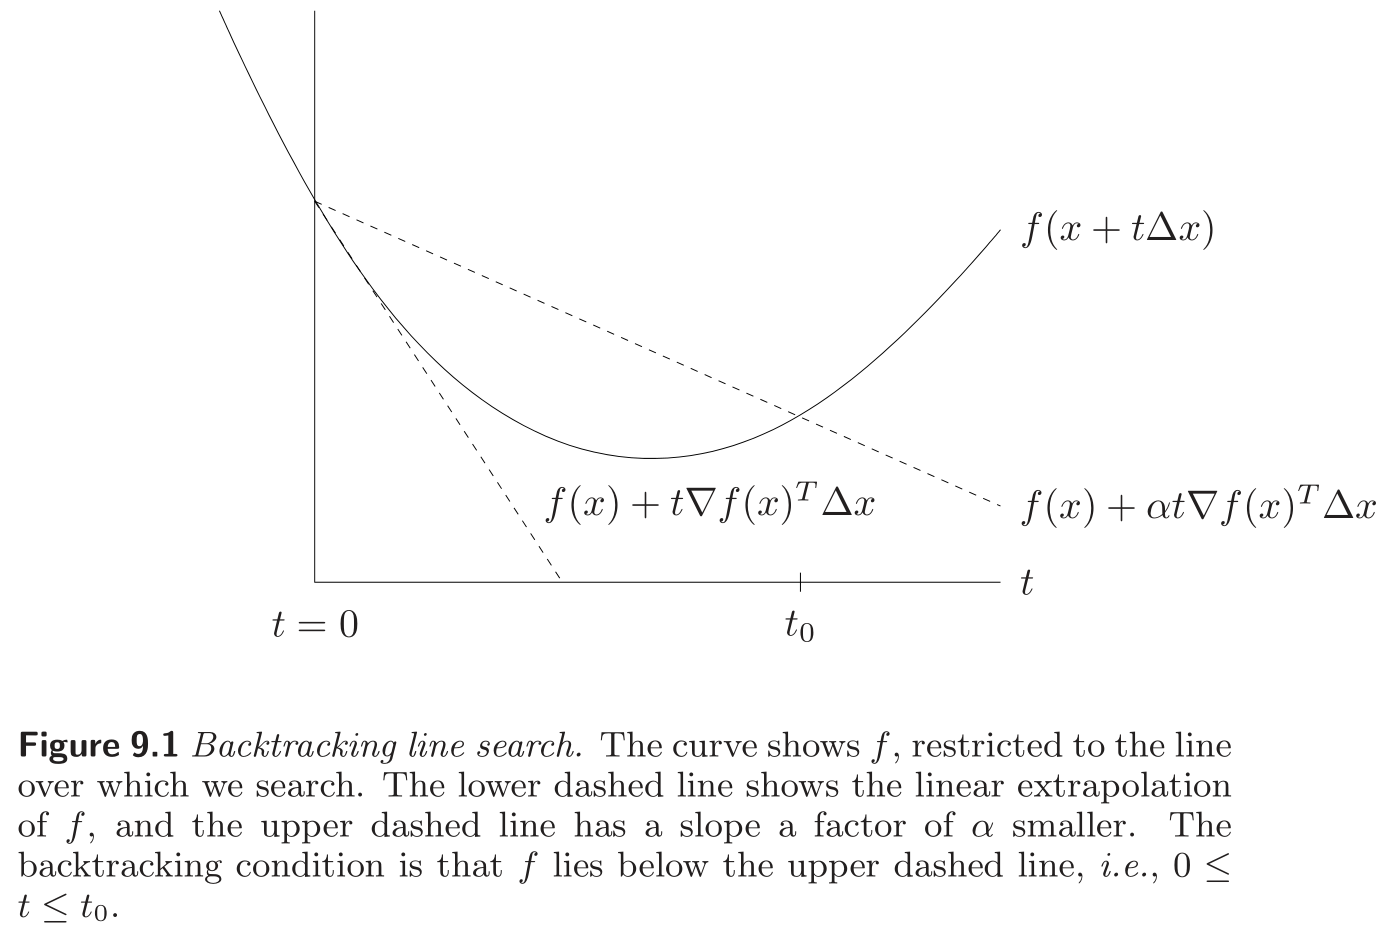
\includegraphics[width=0.75\textwidth]{backtracking_line_search_diagram.png}
\end{center}

Notice that the backtracking search will find a step size $t$ such that $0\leq t\leq t_0$ and that the minimum of the function is in this region. However, the step size we choose may not exactly be the minimum of the function, but we have funneled it down to be closer to the minimum of $f$.
\paragraph{Julia Code}
Here is an implementation of the Backtracking Line Search in Julia with default values for the parameters being $\alpha=0.25$ and $\beta=0.5$.
\begin{jllisting}
	function ln_srch(d_dir,x,f,fx,dfx;alpha=0.25,beta=0.5)
		t = 1
		x1 = x+t*d_dir
		y1 = f(x1)
		y2 = fx+alpha*t*(dfx)'*d_dir
		while y1 > y2
			t = beta*t
			x1 = x+t*d_dir
			y1 = f(x1)
			y2 = fx+alpha*t*(dfx)'*d_dir
		end
		return t
	end
\end{jllisting}
\subsection*{Gradient Descent}
Now we proceed to discuss descent algorithms, the first of which will be the {\color{tiananmen}\textbf{gradient descent method}}.
\begin{algorithm}[H]
	\caption{Gradient Descent Method \cite{Boyd2004}\label{GradientDescentAlg}}
	\begin{algorithmic} 
		\State \textbf{given} a starting point $x\in\textbf{dom}f$.
		\Repeat
		\begin{enumerate}
			\item $\Delta x:=-\nabla f(x)$.
			\item \textit{Line search.} Choose step size $t$ via exact or backtracking line search.
			\item \textit{Update.} $x:=x+t\Delta x$.
		\end{enumerate}
		\Until{stopping criterion is satisfied.}
	\end{algorithmic}
\end{algorithm}
The gradient descent method chooses the search direction to be the negative gradient. That is, in this method we set $\Delta x=-\nabla f(x)$, where $f$ is the function we seek to optimize. Since the gradient of a function gives the direction of greatest increase, naturally the negative gradient will give the direction of the most rapid decline.

Notice that essentially the algorithm uses a line search to determine a step size and then we update our iterate in the direction of the steepest descent. This is repeated until we meet some sort of stopping criterion, typically something of the form $\|\nabla f(x)\|_2\leq\eta$, where $\eta$ is small and positive.

Below is an implementation of the gradient descent algorithm in Julia for a function $f(x,y)=y^3-y+x^2-3x$. This program uses the Backtracking Line Search implementation presented earlier to perform the line search. Notice that we need to input the function, the gradient of the function, and an initial guess.
\begin{jllisting}
	using LinearAlgebra
	
	#Function to Optimize
	f(x)=(x[2])^3-x[2]+(x[1])^2-3x[1]
	
	#Gradient of Function
	df(x)=[2x[1]-3,3x[2]^2-1]
	
	#Initial Point
	x=[0,0]
	
	#Gradient Descent Algorithm
	function grad_d(f,df,x)
		d_dir = -df(x)
		t = ln_srch(d_dir,x,f,f(x),df(x))
		x = x + t*d_dir
		return x
	end
	
	#Compute Minimum for Defined Tolerance
	while norm(df(x))>0.00001
		global x = grad_d(f,df,x)
	end
	
	display(x)
	
\end{jllisting}
\subsection*{Nonlinear Conjugate Gradient Method}
Suppose we have a function $f(x)$ of $N$ variables. Let $x_0$ be an initial guess value for the minimum.

The opposite of the gradient will give the direction of steepest descent. Therefore, we start off by setting $\Delta x_0=-\nabla f(x_0)$.

We set an adjustable step length $\alpha$ and perform a line search in the direction $d_0=\Delta x_0$ until a minimum of $f$ is reached:
\begin{align*}
	&\alpha_0:=\arg\min_{\alpha} f(x_0+\alpha\Delta x_0),\\
	&x_1=x_0+\alpha_0\Delta x_0.
\end{align*}

$\alpha_i$ is found by ensuring that the gradient is orthogonal to the search direction.

After the first iteration, the following steps constitute one iteration along a conjugate direction:
\begin{enumerate}
	\item Calculate the new steepest descent direction: $\Delta x_i=-\nabla f(x_i)$,
	\item Compute $\beta_i$ using some formulation. Two options are below:
	\begin{itemize}
		\item Fletcher--Reeves: $\beta_i^{FR}=\frac{\Delta x_i^T\Delta x_i}{\Delta x_{i=1}^T\Delta x_{i-1}}$
		\item Polak--Ribi\`{e}re: $\beta_{i}^{PR}=\frac{\Delta x_i^T(\Delta x_i-\Delta x_{i-1})}{\Delta x_{i-1}^T\Delta x_{i-1}}$
	\end{itemize}
	\item Update the conjugate direction: $d_i=\Delta x_i+\beta_i d_{i-1}$,
	\item Line search: Optimize $\alpha_i =\arg\min_{\alpha} f(x_i+\alpha d_i)$,
	\item Update iterate value: $x_{i+1}=x_i+\alpha_i d_i$.
\end{enumerate}

The algorithm below uses the Newton-Raphson method to find the values of $\alpha_i$.

Given a function $f$, a starting value $x$, a maximum number of CG iterations $i_{\text{max}}$, a CG error tolerance $\epsilon<1$, a maximum number of Newton-Raphson iterations $j_{\text{max}}$, and a Newton-Raphson error tolerance $\varepsilon<1$:
\begin{algorithm}[H]
	\caption{Nonlinear Conjugate Gradient Using Newton-Raphson \cite{Shewchuk1994}\label{CongGradAlg}}
	\begin{algorithmic}
		\State $i\Leftarrow 0$
		\State $k\Leftarrow 0$
		\State $r\Leftarrow -f^{\prime}(x)$
		\State $d\Leftarrow r$
		\State $\delta_{\text{new}}\Leftarrow r^Tr$
		\State $\delta_0\Leftarrow\delta_{\text{new}}$
		\While{$i<i_{\max}$ and $\delta_{\text{new}}>\epsilon^2\delta_0$}
		\State $j\Leftarrow 0$
		\State $\delta_d\Leftarrow d^Td$
		\While{true}
		\State $\alpha\Leftarrow -\frac{\left[f^{\prime}(x)\right]^Td}{d^Tf^{\prime\prime}(x)d}$
		\State $x\Leftarrow x+\alpha d$
		\State $j\Leftarrow j+1$
		\State $j<j_{\text{max}}$ and $\alpha^2\delta_d>\varepsilon^2$ OR \textbf{Break}
		\EndWhile
		\State $r\Leftarrow -f^{\prime}(x)$
		\State $\delta_{\text{old}}\Leftarrow\delta_{\text{new}}$
		\State $\delta_{\text{new}}\Leftarrow r^T r$
		\State $\beta\Leftarrow\frac{\delta_{\text{new}}}{\delta_{\text{old}}}$
		\State $d\Leftarrow r+\beta d$
		\State $k\Leftarrow k+1$
		\If{$k=n$ or $r^T d\leq 0$}
		\State $d\Leftarrow r$
		\State $k\Leftarrow 0$
		\EndIf
		\State $i\Leftarrow i+1$
		\EndWhile
	\end{algorithmic}
\end{algorithm}
\section*{PDE Methods}
\subsection*{Finite Volume Method}
\begin{quote}
	``The new idea of the {\color{tiananmen}finite volume method} is to first integrate the equation over a small so-called {\color{baystate}control volume}, then use the {\color{baystate}divergence theorem} to convert the volume integral into a {\color{baystate}boundary integral involving fluxes}, before finally approximating these fluxes across the boundaries.'' \cite{Gander2018}
\end{quote}

The Finite Volume Method takes advantage of the Divergence Theorem, so here are two different statements of the theorem:

\begin{thm}[Divergence Theorem (Version 1) \cite{dawkins_2018}]
	Let $E$ be a simple solid region and $S$ the boundary surface of $E$ with positive orientation. Let $\vec{F}$ be a vector field whose components have continuous first order partial derivatives. Then $$\iint\limits_S\vec{F}\cdot\dif\vec{S}=\iiint\limits_E\operatorname{div}\vec{F}\dif V.$$
\end{thm}

\begin{thm}[Divergence Theorem (Version 2) \cite{enwiki:1011407395}]
	Suppose that $V$ is a subset of $\mathbb{R}^n$ which is compact and has a piecewise smooth boundary $S$ (also indicated with $\partial V=S$). If $\mathbf{F}$ is a continuously differentiable vector field defined on a neighborhood of $V$. Then $$\iiint\limits_V\left(\nabla\cdot\mathbf{F}\right)\dif V=\oiint\limits_S\left(\mathbf{F}\cdot\hat{n}\right)\dif S$$
\end{thm}
The left side is a volume integral over $V$ and the right side is a surface integral over the boundary of $V$.

\subsubsection*{Finite Volumes for a General Two-Dimensional Diffusion Equation}
For a scalar function $a(x)$ the {\color{tiananmen}general diffusion equation} is $${\color{baystate}\nabla\cdot\left(a(\mathbf{x})\nabla u\right)=f\quad\text{in }\Omega}.$$

``The finite volume method is designed to discretize such differential operators on arbitrary domains with very general grids.'' \cite{Gander2018}

Given a grid of polygons with vertices $\left\lbrace x_i\right\rbrace\subset\Omega$, we create a set of {\color{tiananmen}\textbf{control volumes}} around each $x_i$ which allows the Finite Volume Method to discritize the PDE. One construction of control volumes is {\color{tiananmen}Voronoi cells}.

\begin{defi}[Voronoi Cell \cite{Gander2018}]
	For a given set of vertices $\left\lbrace x_i\right\rbrace\subset\Omega$ of a mesh, we define the corresponding {\color{baystate}\textbf{Voronoi cells}} $V_i$ by $$V_i=\left\lbrace x\in\Omega : \|x-x_i\|\leq\|x-x_j\|, \forall j\neq i, x_j\text{ neighbor of }x_i\right\rbrace.$$
\end{defi}

Then, using the divergence theorem to convert a volume integral into a surface integral, we integrate the PDE over each control volume $V_i$:

$$\int_{V_i}\nabla\cdot\left(a(\mathbf{x})\nabla u\right)\dif\mathbf{x}=\int_{\partial V_i}a(\mathbf{x})\nabla u\cdot\mathbf{n}\dif s=\int_{V_i}f\dif\mathbf{x}.$$

Then, using some approximation schemes, we obtain a sparce and structured linear system.

``One of the main advantages of the finite volume method is that it can naturally take boundary conditions into account on very general domains.'' \cite{Gander2018}

{\huge \fbox{\textbf{The Optimization Problem}}}

An {\color{tiananmen}\textbf{optimization problem}} has the form
{\color{baystate}
\begin{equation}
	\begin{tabular}{lll}
		\text{minimize }   & $f_0(x)$          & \\
		\text{subject to } & $f_i(x)\leq 0$, & $i=1,\ldots, m$\\
						   & $h_i(x) = 0$,      & $i=1,\ldots, p$
	\end{tabular}\label{Optimization}
\end{equation}
}
where
\begin{itemize}
	\item {\color{baystate} $x=\left(x_1,\ldots,x_n\right)$} is the {\color{tiananmen} \textbf{optimization variable}}
	\item {\color{baystate} $f_0 : \mathbb{R}^n\rightarrow\mathbb{R}$} is the {\color{tiananmen} \textbf{objective function}}
	\item {\color{baystate} $f_i : \mathbb{R}^n\rightarrow\mathbb{R}$} are the {\color{tiananmen} \textbf{inequality constraint functions}}
	\item {\color{baystate} $h_i : \mathbb{R}^n\rightarrow\mathbb{R}$} are the {\color{tiananmen}\textbf{equality constraint functions}}
\end{itemize}

If there are no constraints ($m=p=0$), then the problem is called {\color{tiananmen}unconstrained}.

A vector {\color{baystate} $x^\star$} is called {\color{tiananmen} \textbf{optimal}} or a {\color{tiananmen} \textbf{solution}} if it has the smallest objective value among all vectors that satisfy the constraints. That is, $x^\star$ is a solution to the optimization problem if {\color{baystate} for any $z$ with $f_1(z)\leq 0,\ldots, f_m(z)\leq 0$, then $f_0(z)\geq f_0(x^\star)$}.

A point $x$ that is in the domain of all of the functions $f_i$ and $h_i$ is called {\color{tiananmen}\textbf{feasible}} if it satisfies all the constraints. The {\color{tiananmen} \textbf{optimal value}} {\color{baystate}$p^\star$} of the problem is defined as {\color{baystate}$$p^\star=\left\lbrace f_0(x) \mid f_i(x)\leq 0, i=1,\ldots,m, h_i(x)=0, i=1,\ldots,p\right\rbrace.$$}
The optimization problem is {\color{tiananmen}\textbf{linear}} or called a {\color{tiananmen}\textbf{linear program}} if the objective and constraint functions are all linear. That is, {\color{baystate} for $i=1,\ldots,m$, $f_i(\alpha x+\beta y)=\alpha f_i(x)+\beta f_i(y)$ for all $x,y\in\mathbb{R}^n$ and all $\alpha,\beta\in\mathbb{R}$}.

If the optimization problem is not linear, we call it a {\color{tiananmen}\textbf{nonlinear program}}.

We can change a minimization problem into a {\color{tiananmen}\textbf{maximization problem}} by minimizing {\color{baystate}$-f_0$} subject to the same constraints.

\section*{Convex Optimization}

A set {\color{baystate}$C$} is {\color{tiananmen}\textbf{convex}} if the line segment between any two points in $C$ lies in $C$. That is {\color{baystate}if for any $x_1,x_2\in C$ and any $\theta$ with $0\leq\theta\leq 1$, we have $\theta x_1+(1-\theta)x_2\in C$}.

A function {\color{baystate}$f : \mathbb{R}^n\rightarrow\mathbb{R}$} is {\color{tiananmen}\textbf{convex}} if $\mathbf{dom}f$ is a convex set and if for all $x,y\in\mathbf{dom}f$, and $\theta$ with $0\leq\theta\leq 1$, we have
{\color{baystate}
	\begin{equation}
		f\left(\theta x+\left(1-\theta\right)y\right)\leq\theta f(x)+(1-\theta)f(y).
		\label{Convexity}
	\end{equation}
}
A {\color{tiananmen} \textbf{convex optimization problem}} is an optimization problem of the form
{\color{baystate}
	\begin{equation}
		\begin{tabular}{lll}
			\text{minimize }   & $f_0(x)$          & \\
			\text{subject to } & $f_i(x)\leq 0$, & $i=1,\ldots, m$\\
			& $a_i^T = b_i$,      & $i=1,\ldots, p$
		\end{tabular}\label{ConvexOptimization}
	\end{equation}
where $f_0,\ldots,f_m$ are convex functions.
}

There are three additional requirements that differentiate a convex optimization problem versus are regular optimization problem:
{\color{baystate}
\begin{itemize}
	\item the objective function must be convex
	\item the inequality constraint functions must be convex
	\item the equality constraint functions must be {\color{tiananmen}\textbf{affine}}
\end{itemize}
}

In a convex optimization problem we minimize a convex objective function over a convex set.

\textbf{In a convex optimization problem, any {\color{tiananmen}\textbf{locally optimal point}} is also {\color{tiananmen}\textbf{globally optimal}}.}

\section*{The Linear Optimization Problem}

When the objective and constraint functions are all affine, we have a {\color{tiananmen}\textbf{linear optimization problem}} or {\color{tiananmen}\textbf{linear program}}.
{\color{baystate}
	\begin{equation}
		\begin{tabular}{ll}
			\text{minimize }   & $c^Tx+d$       \\
			\text{subject to } & $Gx\preceq h$, \\
			& $Ax=b,$      
		\end{tabular}\label{LinearOptimization}
	\end{equation}
where $G\in\mathbb{R}^{m\times n}$ and $A\in\mathbb{R}^{p\times n}$.} ($\preceq$ represents componentwise inequality.)

Linear optimization problems are convex optimization problems.


\section*{The Quadratic Optimization Problem}

If the objective function is a convex quadratic and the constraint functions are affine in (\ref{ConvexOptimization}), then we have a {\color{tiananmen}\textbf{quadratic program}}.

{\color{baystate}
	\begin{equation}
		\begin{tabular}{ll}
			\text{minimize} & $\frac{1}{2}x^TPx+q^Tx+r$ \\
			\text{subject to} & $Gx\preceq h$\\
			& $Ax=b,$
		\end{tabular}\label{QuadraticOptimization}
	\end{equation}
where $P$ is a symmetric positive semidefinite $n\times n$ matrix, $G\in\mathbb{R}^{m\times n}$,  $A\in\mathbb{R}^{p\times n}$, $q\in\mathbb{R}^n$, and $r\in\mathbb{R}$}.

\subsection*{Example: Least-Squares}

In the {\color{tiananmen}\textbf{least squares problem}} we want to minimize {\color{baystate}$\|Ax-b\|_2$}. Notice {\color{baystate}$$\frac{1}{2}\|Ax-b\|_2^2=\frac{1}{2}x^TA^TAx-b^TAx+\frac{1}{2}b^Tb$$} is actually a convex quadratic function. Since $\|Ax-b\|_2\geq 0$, we know that the minimal solution for $\frac{1}{2}\|Ax-b\|_2^2$ will also be a minimal solution for $\|Ax-b\|_2$. Therefore, if we are able to minimize the corresponding quadratic function, we will have accomplished our goal.

Looking back to (\ref{QuadraticOptimization}), we have $P=A^TA$, $q=b^TA$, and $r=\frac{1}{2}b^Tb$, so this is really a quadratic optimization problem.
\\

{\huge \fbox{\textbf{The Method of Moving Asymptotes (MMA)}}}

\begin{quote}
	``Ideally, a method for structural optimization should be flexible and general. It should be able to handle not only element sizes as design variables, but also, for instance, shape variables and material orientation angles.''\cite{Svanberg1987}
\end{quote}

\section*{General Method Description}
Consider a structural optimization problem of the following general form

{\color{baystate}
	\begin{equation}
		\begin{tabular}{llll}
			$P$: & minimize & $f_0(\mathbf{x})$ & $\left(\mathbf{x}\in\mathbb{R}^n\right)$ \\
			& subject to & $f_i(\mathbf{x})\leq\hat{f}_i$, & for $i=1,\ldots,m$ \\
			&  & $\underline{x}_j\leq x_j\leq \overline{x}_j$, & for $j=1,\ldots,n$
		\end{tabular}
	\end{equation}
}
where
\begin{itemize}
	\item $\mathbf{x}=\left(x_1,\ldots,x_n\right)^T$ is the vector of {\color{tiananmen}design variables}
	\item $f_0(\mathbf{x})$ is the {\color{tiananmen}objective function} (typically structural weight)
	\item $f_i(\mathbf{x})\leq\hat{f}_i$ are {\color{tiananmen}behavior constraints} (typically limitations on stresses and displacements)
	\item $\underline{x}_j$ and $\overline{x}_j$ are given {\color{tiananmen}lower and upper bounds} (``technological constraints'') {\color{tiananmen}on the design variables}
\end{itemize}

The general approach for solving such optimization problems is to split it up and solve a sequence of subproblems using the following iteration:
{\color{baystate}
\begin{description}
	\item[\textbf{\underline{Step 0}:}] Choose a starting point $\mathbf{x}^{(0)}$, and let the iteration index $k=0$.
	\item[\textbf{\underline{Step 1}:}] Given an iteration point $\mathbf{x}^{(k)}$, calculate $f_i(\mathbf{x}^{(k)})$ and the gradients $\nabla f_i(\mathbf{x}^{(k)})$ for $i=0,1,\ldots,m$.
	\item[\textbf{\underline{Step 2}:}] Generate a subproblem $P^{(k)}$ by replacing, in $(6)$, the (usually implicit) functions $f_i$ by approximating explicit functions $f_i^{(k)}$, based on calculations from Step 1.
	\item[\textbf{\underline{Step 3}:}] Solve $P^{(k)}$ and let the optimal solution of this subproblem be the next iteration point $\mathbf{x}^{(k+1)}$. Let $k=k+1$ and go to Step 1.
\end{description}
}

In MMA, each $f_i^{(k)}$ is obtained by a linearization of $f_i$ in variables of the type $$\frac{1}{x_j-L_j}\quad\text{or}\quad\frac{1}{U_j-x_j}$$ dependent on the signs of the derivatives of $f_i$ at $\mathbf{x}^{(k)}$. The values of $L_j$ and $U_j$ are normally changed between iterations and are referred to as {\color{tiananmen}moving asymptotes}.

\subsection*{Defining The Functions $f_i^{(k)}$}

Given the iteration point $\mathbf{x}^{(k)}$ at an iteration $k$, values of the parameters $L_j^{(k)}$ and $U_j^{(k)}$ are chosen, for $j=1,\ldots,n$, such that $L_j^{(k)}<x_j^{(k)}<U_j^{(k)}$.

{\color{baystate}
For each $i=0,1,\ldots,m$, $f_i^{(k)}$ is defined by $$f_i^{(k)}(\mathbf{x})=r_i^{(k)}+\sum\limits_{j=1}^{n}\left(\frac{p_{ij}^{(k)}}{U_j^{(k)}-x_j}+\frac{q_{ij}^{(k)}}{x_j-L_j^{(k)}}\right)$$
where
$$p_{ij}^{(k)}=\begin{cases}
	\left(U_j^{(k)}-x_j^{(k)}\right)^2, & \text{if }\frac{\partial f_i}{\partial x_j}>0\\
	0, & \text{if }\frac{\partial f_i}{\partial x_j}\leq 0
\end{cases}$$

$$q_{ij}^{(k)}=\begin{cases}
	0, & \text{if }\frac{\partial f_i}{x_j}\geq 0\\
	-\left(x_j^{(k)}-L_j^{(k)}\right)^2\frac{\partial f_i}{\partial x_j}, & \text{if }\frac{\partial f_i}{\partial x_j}<0
\end{cases}$$

$$r_i^{(k)}=f_i(\mathbf{x}^{(k)})-\sum\limits_{j=1}^{n}\left(\frac{p_{ij}^{(k)}}{U_j^{(k)}-x_j^{(k)}}+\frac{q_{ij}^{(k)}}{x_j^{(k)}-L_j^{(k)}}\right)$$

and where all $\frac{\partial f_i}{\partial x_j}$ are evaluated at $\mathbf{x}=\mathbf{x}^{(k)}$.
}

Notice that $f_i^{(k)}$ is a first-order approximation of $f_i$ at $\mathbf{x}^{(k)}$. Additionally, by construction, $f_i^{(k)}$ is a {\color{tiananmen}convex function}.

Looking at the second derivatives, the closer $L_j^{(k)}$ and $U_j^{(k)}$ are chosen to $x_j^{(k)}$, the larger the second derivatives become and hence the more curvature is given to the approximating function $f_i^{(k)}$. This means that the closer $L_j^{(k)}$ and $U_j^{(k)}$ are chosen to $x_j^{(k)}$, the more conservative becomes the approximation of the original problem. If $L^{(k)}$ and $U^{(k)}$ are chosen `far away' from $\mathbf{x}^{(k)}$, then the approximation $f_i^{(k)}$ becomes close to linear.

We always choose the values of $L_j^{(k)}$ and $U_j^{(k)}$ to be finite. As a result each $f_i^{(k)}$ becomes strictly convex except when $\frac{\partial f_i}{\partial x_j}=0$ at $\mathbf{x}=x^{(k)}$.

Now, with the approximating functions $f_i^{(k)}$ as defined earlier, we have the following subproblem $P^{(k)}$:

{\color{baystate}
	\begin{equation}
		\begin{tabular}{llll}
			$P^{(k)}$: & minimize & $\sum\limits_{j=1}^{n}\left(\frac{p_{oj}^{(k)}}{U_j^{(k)}-x_j}+\frac{q_{oj}^{(k)}}{x_j-L_j^{(k)}}\right)+r_o^{(k)}$ &  \\
			& subject to & $\sum\limits_{j=1}^{n}\left(\frac{p_{ij}^{(k)}}{U_j^{(k)}-x_j}+\frac{q_{ij}^{(k)}}{x_j-L_j^{(k)}}\right)+r_i^{(k)}\leq\hat{f}_i$, & for $i=1,\ldots,m$ \\
			& and & $\max\lbrace\underline{x}_j,\alpha_j^{(k)}\rbrace\leq x_j\leq \min\lbrace \overline{x}_j,\beta_j^{(k)}\rbrace$, & for $j=1,\ldots,n$
		\end{tabular}
	\end{equation}
}

(The parameters $\alpha_j^{(k)}$ and $\beta_j^{(k)}$ are called ``{\color{tiananmen}move limits}'' and are not that important.)

$\alpha_j^{(k)}$ and $\beta_j^{(k)}$ should at least be chosen such that $L_j^{(k)}<\alpha_j^{(k)}<x_j^{(k)}<\beta_j^{(k)}<U_j^{(k)}$.

\subsubsection*{\underline{General Rule for how to choose $L_j^{(k)}$ and $U_j^{(k)}$}:}
\begin{itemize}
	\item[(a)] If the process tends to oscillate, then it needs to be stabilized and this can be accomplished by moving the asymptotes closer to the current iteration point.
	\item[(b)] If, instead, the process is monotone and slow, it needs to be ``relaxed''. This can be accomplished by moving the asymptotes away from the current iteration point.
\end{itemize}

\subsection*{The Dual Problem}

$P^{(k)}$ is a convex, separable problem, so we can create a dual problem using a Lagrangian function. The Lagrangian function corresponding to $P^{(k)}$ is given by 
{\color{baystate}
	$$\ell(x,y)=f_0^{(k)}(\mathbf{x})+\sum\limits_{i=1}^{m}y_if_i^{(k)}(\mathbf{x})$$
}

Letting $\mathbf{y}$ be the vector of {\color{tiananmen}Lagrange multipliers} or ``dual variables'' and doing some derivations, we get the {\color{tiananmen}dual objective function} $W$ defined (for $\mathbf{y}\geq 0$), as below:
{\color{baystate}
	\begin{align*}
		W(\mathbf{y})&=\min\limits_x\lbrace\ell(\mathbf{x},\mathbf{y}); \alpha_j\leq x_j\leq \beta_j\text{ for all }j\rbrace\\
		&=r_0-\mathbf{y}^T\mathbf{b}+\sum\limits_{j=1}^{n}W_j(\mathbf{y})
	\end{align*}
	where $W_j(\mathbf{y})=\min\limits_{x_j}\lbrace l_j(x_j,\mathbf{y}); \alpha_j\leq x_j\leq \beta_j\rbrace$
}

This formulation is beneficial since it ``eliminates'' $\mathbf{x}$.

The dual problem corresponding to $P^{(k)}$ is given as follows:

{\color{baystate}
\begin{equation}
	\begin{tabular}{lll}
		$D$: & maximize & $W(\mathbf{y})$\\
		     & subject to & $\mathbf{y}\geq 0$
	\end{tabular}
\end{equation}
}

$D$ is a ``nice'' problem which may be solved by an arbitrary gradient method.

Once the dual problem has been solved the optimal solution of the primal subproblem $P^{(k)}$ is directly obtained by just pluggin in the optimal dual solution $\mathbf{y}$ in to the following expression:
{\color{baystate}
$$x_j(\mathbf{y})=\frac{\left(p_{0j}+\mathbf{y}^T\mathbf{p}_j\right)^{1/2}L_j+\left(q_{0j}+\mathbf{y}^T\mathbf{q}_j\right)^{1/2}U_j}{\left(p_{0j}+\mathbf{y}^T\mathbf{p}_j\right)^{1/2}+\left(q_{0j}+\mathbf{y}^T\mathbf{q}_j\right)^{1/2}}.$$
}

{\huge \fbox{\textbf{The SIMP Method}}}

\bibliographystyle{siam}
\bibliography{Research_Log.bib}
\nocite{Boyd2004}
\nocite{Gander2018}
\nocite{dawkins_2018}
\nocite{enwiki:1011407395}
\nocite{Shewchuk1994}
\nocite{Svanberg1987}

\end{document}